%!TEX root = ../template.tex
%%%%%%%%%%%%%%%%%%%%%%%%%%%%%%%%%%%%%%%%%%%%%%%%%%%%%%%%%%%%%%%%%%%%
%% chapter4.tex
%% NOVA thesis document file
%%
%% Chapter with lots of dummy text
%%%%%%%%%%%%%%%%%%%%%%%%%%%%%%%%%%%%%%%%%%%%%%%%%%%%%%%%%%%%%%%%%%%%

\typeout{NT FILE chapter4.tex}%

\chapter{Planning}
\label{cha:Planning}

This chapter outlines the timeline and milestones for the development of the proposed AI-driven tool. The planning process is structured to ensure efficient progress across all stages, from initial data collection and preprocessing to model development, evaluation, and deployment. A detailed Gantt chart is provided to visualize the schedule.
\section{Timeline \& Milestones}
The timeline is designed to accommodate iterative refinement and unforeseen challenges, ensuring a robust and reliable outcome.

\begin{figure}[h]
    \centering
    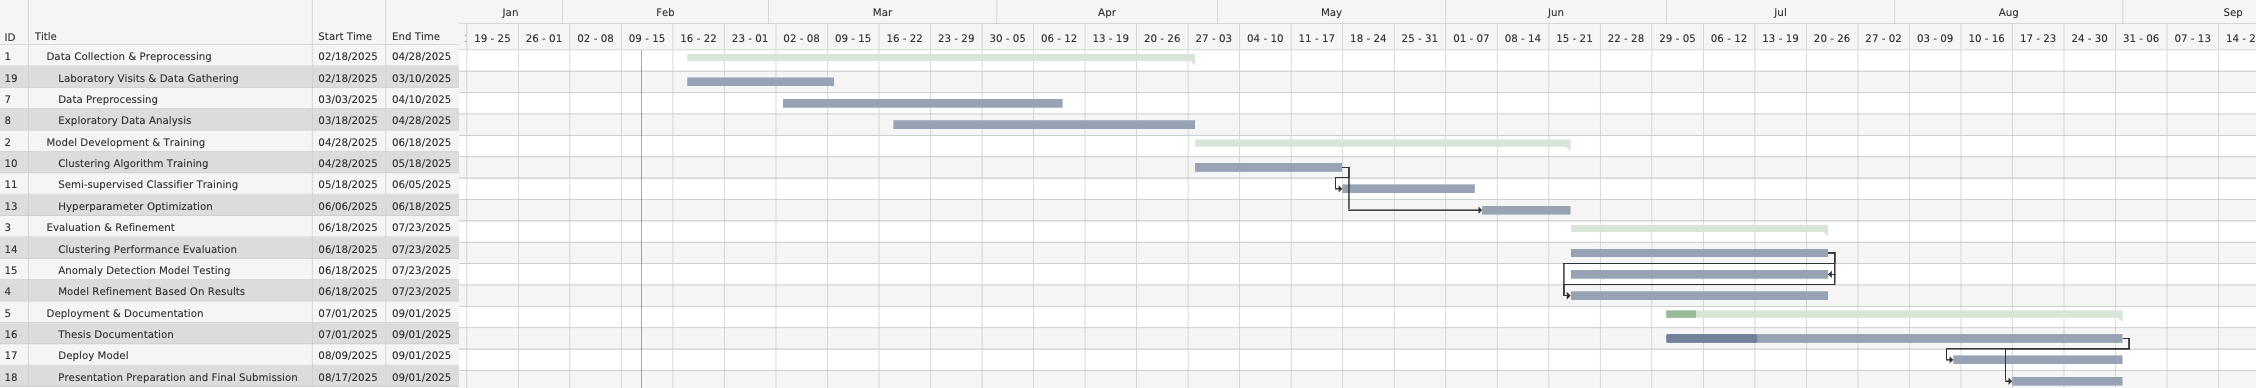
\includegraphics[width=\textwidth]{gantt2.png} 
    \caption{Gantt Chart of the Project Timeline}
    \label{fig:gantt}
\end{figure}

The Gantt chart (Figure \ref{fig:gantt}) illustrates the following phases:
\begin{itemize}
\item \textbf{Phase 1:} Data Collection \& Preprocessing (Weeks 1–10)
\item \textbf{Phase 2:} Model Development \& Training (Weeks 10–17)
\item \textbf{Phase 3:} Evaluation \& Refinement (Weeks 17–22)
\item \textbf{Phase 4:} Deployment \& Documentation (Weeks 19–27)
\end{itemize}